% Options for packages loaded elsewhere
\PassOptionsToPackage{unicode}{hyperref}
\PassOptionsToPackage{hyphens}{url}
%
\documentclass[
  man]{apa6}
\usepackage{amsmath,amssymb}
\usepackage{lmodern}
\usepackage{iftex}
\ifPDFTeX
  \usepackage[T1]{fontenc}
  \usepackage[utf8]{inputenc}
  \usepackage{textcomp} % provide euro and other symbols
\else % if luatex or xetex
  \usepackage{unicode-math}
  \defaultfontfeatures{Scale=MatchLowercase}
  \defaultfontfeatures[\rmfamily]{Ligatures=TeX,Scale=1}
\fi
% Use upquote if available, for straight quotes in verbatim environments
\IfFileExists{upquote.sty}{\usepackage{upquote}}{}
\IfFileExists{microtype.sty}{% use microtype if available
  \usepackage[]{microtype}
  \UseMicrotypeSet[protrusion]{basicmath} % disable protrusion for tt fonts
}{}
\makeatletter
\@ifundefined{KOMAClassName}{% if non-KOMA class
  \IfFileExists{parskip.sty}{%
    \usepackage{parskip}
  }{% else
    \setlength{\parindent}{0pt}
    \setlength{\parskip}{6pt plus 2pt minus 1pt}}
}{% if KOMA class
  \KOMAoptions{parskip=half}}
\makeatother
\usepackage{xcolor}
\usepackage{graphicx}
\makeatletter
\def\maxwidth{\ifdim\Gin@nat@width>\linewidth\linewidth\else\Gin@nat@width\fi}
\def\maxheight{\ifdim\Gin@nat@height>\textheight\textheight\else\Gin@nat@height\fi}
\makeatother
% Scale images if necessary, so that they will not overflow the page
% margins by default, and it is still possible to overwrite the defaults
% using explicit options in \includegraphics[width, height, ...]{}
\setkeys{Gin}{width=\maxwidth,height=\maxheight,keepaspectratio}
% Set default figure placement to htbp
\makeatletter
\def\fps@figure{htbp}
\makeatother
\setlength{\emergencystretch}{3em} % prevent overfull lines
\providecommand{\tightlist}{%
  \setlength{\itemsep}{0pt}\setlength{\parskip}{0pt}}
\setcounter{secnumdepth}{-\maxdimen} % remove section numbering
% Make \paragraph and \subparagraph free-standing
\ifx\paragraph\undefined\else
  \let\oldparagraph\paragraph
  \renewcommand{\paragraph}[1]{\oldparagraph{#1}\mbox{}}
\fi
\ifx\subparagraph\undefined\else
  \let\oldsubparagraph\subparagraph
  \renewcommand{\subparagraph}[1]{\oldsubparagraph{#1}\mbox{}}
\fi
\newlength{\cslhangindent}
\setlength{\cslhangindent}{1.5em}
\newlength{\csllabelwidth}
\setlength{\csllabelwidth}{3em}
\newlength{\cslentryspacingunit} % times entry-spacing
\setlength{\cslentryspacingunit}{\parskip}
\newenvironment{CSLReferences}[2] % #1 hanging-ident, #2 entry spacing
 {% don't indent paragraphs
  \setlength{\parindent}{0pt}
  % turn on hanging indent if param 1 is 1
  \ifodd #1
  \let\oldpar\par
  \def\par{\hangindent=\cslhangindent\oldpar}
  \fi
  % set entry spacing
  \setlength{\parskip}{#2\cslentryspacingunit}
 }%
 {}
\usepackage{calc}
\newcommand{\CSLBlock}[1]{#1\hfill\break}
\newcommand{\CSLLeftMargin}[1]{\parbox[t]{\csllabelwidth}{#1}}
\newcommand{\CSLRightInline}[1]{\parbox[t]{\linewidth - \csllabelwidth}{#1}\break}
\newcommand{\CSLIndent}[1]{\hspace{\cslhangindent}#1}
\ifLuaTeX
\usepackage[bidi=basic]{babel}
\else
\usepackage[bidi=default]{babel}
\fi
\babelprovide[main,import]{english}
% get rid of language-specific shorthands (see #6817):
\let\LanguageShortHands\languageshorthands
\def\languageshorthands#1{}
% Manuscript styling
\usepackage{upgreek}
\captionsetup{font=singlespacing,justification=justified}

% Table formatting
\usepackage{longtable}
\usepackage{lscape}
% \usepackage[counterclockwise]{rotating}   % Landscape page setup for large tables
\usepackage{multirow}		% Table styling
\usepackage{tabularx}		% Control Column width
\usepackage[flushleft]{threeparttable}	% Allows for three part tables with a specified notes section
\usepackage{threeparttablex}            % Lets threeparttable work with longtable

% Create new environments so endfloat can handle them
% \newenvironment{ltable}
%   {\begin{landscape}\centering\begin{threeparttable}}
%   {\end{threeparttable}\end{landscape}}
\newenvironment{lltable}{\begin{landscape}\centering\begin{ThreePartTable}}{\end{ThreePartTable}\end{landscape}}

% Enables adjusting longtable caption width to table width
% Solution found at http://golatex.de/longtable-mit-caption-so-breit-wie-die-tabelle-t15767.html
\makeatletter
\newcommand\LastLTentrywidth{1em}
\newlength\longtablewidth
\setlength{\longtablewidth}{1in}
\newcommand{\getlongtablewidth}{\begingroup \ifcsname LT@\roman{LT@tables}\endcsname \global\longtablewidth=0pt \renewcommand{\LT@entry}[2]{\global\advance\longtablewidth by ##2\relax\gdef\LastLTentrywidth{##2}}\@nameuse{LT@\roman{LT@tables}} \fi \endgroup}

% \setlength{\parindent}{0.5in}
% \setlength{\parskip}{0pt plus 0pt minus 0pt}

% Overwrite redefinition of paragraph and subparagraph by the default LaTeX template
% See https://github.com/crsh/papaja/issues/292
\makeatletter
\renewcommand{\paragraph}{\@startsection{paragraph}{4}{\parindent}%
  {0\baselineskip \@plus 0.2ex \@minus 0.2ex}%
  {-1em}%
  {\normalfont\normalsize\bfseries\itshape\typesectitle}}

\renewcommand{\subparagraph}[1]{\@startsection{subparagraph}{5}{1em}%
  {0\baselineskip \@plus 0.2ex \@minus 0.2ex}%
  {-\z@\relax}%
  {\normalfont\normalsize\itshape\hspace{\parindent}{#1}\textit{\addperi}}{\relax}}
\makeatother

% \usepackage{etoolbox}
\makeatletter
\patchcmd{\HyOrg@maketitle}
  {\section{\normalfont\normalsize\abstractname}}
  {\section*{\normalfont\normalsize\abstractname}}
  {}{\typeout{Failed to patch abstract.}}
\patchcmd{\HyOrg@maketitle}
  {\section{\protect\normalfont{\@title}}}
  {\section*{\protect\normalfont{\@title}}}
  {}{\typeout{Failed to patch title.}}
\makeatother

\usepackage{xpatch}
\makeatletter
\xapptocmd\appendix
  {\xapptocmd\section
    {\addcontentsline{toc}{section}{\appendixname\ifoneappendix\else~\theappendix\fi\\: #1}}
    {}{\InnerPatchFailed}%
  }
{}{\PatchFailed}
\keywords{keywords\newline\indent Word count: X}
\DeclareDelayedFloatFlavor{ThreePartTable}{table}
\DeclareDelayedFloatFlavor{lltable}{table}
\DeclareDelayedFloatFlavor*{longtable}{table}
\makeatletter
\renewcommand{\efloat@iwrite}[1]{\immediate\expandafter\protected@write\csname efloat@post#1\endcsname{}}
\makeatother
\usepackage{lineno}

\linenumbers
\usepackage{csquotes}
\ifLuaTeX
  \usepackage{selnolig}  % disable illegal ligatures
\fi
\IfFileExists{bookmark.sty}{\usepackage{bookmark}}{\usepackage{hyperref}}
\IfFileExists{xurl.sty}{\usepackage{xurl}}{} % add URL line breaks if available
\urlstyle{same} % disable monospaced font for URLs
\hypersetup{
  pdftitle={20 to 18 - Final Scale Definitions of the Bifactor Engagement Scale},
  pdfauthor={First Author1 \& Ernst-August Doelle1,2},
  pdflang={en-EN},
  pdfkeywords={keywords},
  hidelinks,
  pdfcreator={LaTeX via pandoc}}

\title{20 to 18 - Final Scale Definitions of the Bifactor Engagement Scale}
\author{First Author\textsuperscript{1} \& Ernst-August Doelle\textsuperscript{1,2}}
\date{}


\shorttitle{20 to 18}

\authornote{

Add complete departmental affiliations for each author here. Each new line herein must be indented, like this line.

Enter author note here.

The authors made the following contributions. First Author: Conceptualization, Writing - Original Draft Preparation, Writing - Review \& Editing; Ernst-August Doelle: Writing - Review \& Editing, Supervision.

Correspondence concerning this article should be addressed to First Author, Postal address. E-mail: \href{mailto:my@email.com}{\nolinkurl{my@email.com}}

}

\affiliation{\vspace{0.5cm}\textsuperscript{1} Wilhelm-Wundt-University\\\textsuperscript{2} Konstanz Business School}

\abstract{%
We finalize the scale definitions for a bifactor engagement measure that is comprised of intentionally complex items.
}



\begin{document}
\maketitle

\hypertarget{methods}{%
\section{Methods}\label{methods}}

\hypertarget{participants}{%
\subsection{Participants}\label{participants}}

Of the 743 total Qualtrics panel respondents, 366 were excluded based on conservative indices of carelessness across the larger survey (consistent non-differentiating responses across more than 20 consecutive items or greater than 50\% missing responses. For Prolific panel respondents, 568 were retained of 785 total participants due to the same exclusion criteria. The smaller (\emph{n} = 232) snowball sample retained all participants for a total combined analysis sample of 1177.

\hypertarget{material}{%
\subsection{Material}\label{material}}

\hypertarget{procedure}{%
\subsection{Procedure}\label{procedure}}

A previous instrument administration reduced 36 candidate items to 20. Primarily for reason of equal balance, we wanted to ultimately land on 18 items (6 per attitudinal/substantive scale dimension, 2 per bifactor subscale). Two primary considerations were given to the decision to retain or delete the 6 deletion candidates: 1) is the content of the item necessary for the definitional content domain, and 2) does the empirical functioning of the item implicate possible revision/deletion. The items considered deletion candidates were from the Absorption-Cognition subscale (Item 1: \emph{I am able to concentrate on my work without getting distracted}, Item 3: \emph{Time passes quickly while I'm working}, and Item 4: \emph{I find it difficult to mentally disconnect from work}) and the Dedication-Cognition subscale (Item 25: \emph{I plan to stay with this company as my career advances}, Item 26: \emph{I believe this company cares about my career goals}, and Item 28: \emph{This organization challenges me to work at my full potential}).

\hypertarget{data-analysis}{%
\subsection{Data analysis}\label{data-analysis}}

We used R (Version 4.2.1; R Core Team, 2022) and the R-packages \emph{careless} (Version 1.2.1; Yentes \& Wilhelm, 2021), \emph{descr} (Version 1.1.5; Dirk Enzmann, Schwartz, Jain, \& Kraft, 2021), \emph{lavaan} (Version 0.6.12; Rosseel, 2012), \emph{papaja} (Version 0.1.1; Aust \& Barth, 2022), and \emph{tinylabels} (Version 0.2.3; Barth, 2022) for all our analyses.

\begin{figure}
\centering
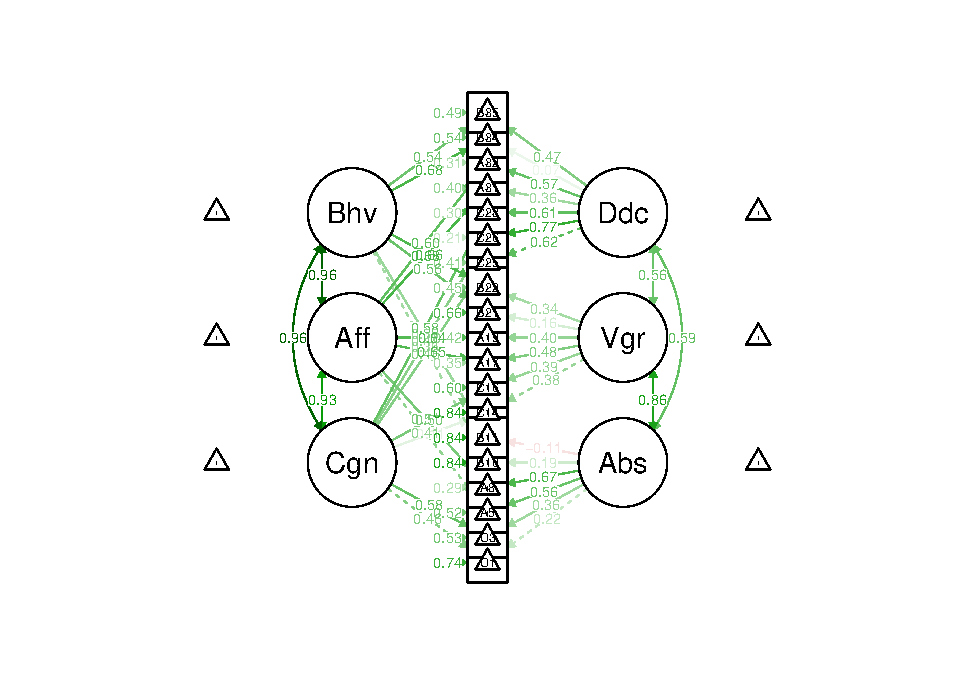
\includegraphics{20to18_files/figure-latex/scalereduction-1.pdf}
\caption{\label{fig:scalereduction}Bifactor analysis minus Item 4.}
\end{figure}

Looking first at the Absorption-Cognition candidate items, Item 4 stood out as a candidate for exclusion based on empirical indices (corrected item-total correlations, inter-item correlations, and bifactor analysis fit {[}\(\chi^2_{with}\) = 676.51, \(\chi^2_{without}\) = 499.05{]}). Conceptually we also agreed that Item 4 was not uniquely critical for comprehensive coverage across either the Cognition or Absorption constructs. Figure \ref{fig:scalereduction} presents the visual CFA.

\hypertarget{results}{%
\section{Results}\label{results}}

\begin{lltable}

\begin{longtable}{llll}\noalign{\getlongtablewidth\global\LTcapwidth=\longtablewidth}
\caption{\label{tab:itemstable}Suggested final scale definitions.}\\
\toprule
Substantive & \multicolumn{1}{c}{Attitudinal} & \multicolumn{1}{c}{Item.Number} & \multicolumn{1}{c}{Item.Stem}\\
\midrule
\endfirsthead
\caption*{\normalfont{Table \ref{tab:itemstable} continued}}\\
\toprule
Substantive & \multicolumn{1}{c}{Attitudinal} & \multicolumn{1}{c}{Item.Number} & \multicolumn{1}{c}{Item.Stem}\\
\midrule
\endhead
Absorption & Cognitive & 1 & I am able to concentrate on my work without getting distracted\\
Absorption & Cognitive & 3 & Time passes quickly while I'm working\\
Absorption & Affective & 5 & I enjoy thinking about work even when I'm not at work\\
Absorption & Affective & 8 & I love starting my workday\\
Absorption & Behavioral & 10 & I have to be reminded to take breaks while I'm at work\\
Absorption & Behavioral & 11 & I never miss a work deadline\\
Vigor & Cognitive & 14 & Thinking about work saps my energy\\
Vigor & Cognitive & 16 & I'm able to maintain good levels of energy throughout the workday\\
Vigor & Affective & 17 & I enjoy spending time completing my job tasks\\
Vigor & Affective & 19 & I feek motivated to go beyond what is asked of me at work\\
Vigor & Behavioral & 21 & When work is slow I find ways to be productive\\
Vigor & Behavioral & 22 & I express enthusiasm for my job while at work\\
Dedication & Cognitive & 25 & I plan to stay with this company as my career advances\\
Dedication & Cognitive & 26 & I believe this company cares about my career goals\\
Dedication & Cognitive & 28 & This organization challenges me to work at my full potential\\
Dedication & Affective & 31 & I feel proud of my accomplishments within this organization\\
Dedication & Affective & 32 & My job makes me feel like I'm part of something meaningful\\
Dedication & Behavioral & 34 & I embrace challenging situations at work\\
Dedication & Behavioral & 35 & I speak positively about this organization to others\\
\bottomrule
\end{longtable}

\end{lltable}

The final recommended scale definitions are located in Table \ref{tab:itemstable}.

\hypertarget{discussion}{%
\section{Discussion}\label{discussion}}

\newpage

\hypertarget{references}{%
\section{References}\label{references}}

\hypertarget{refs}{}
\begin{CSLReferences}{1}{0}
\leavevmode\vadjust pre{\hypertarget{ref-R-papaja}{}}%
Aust, F., \& Barth, M. (2022). \emph{{papaja}: {Prepare} reproducible {APA} journal articles with {R Markdown}}. Retrieved from \url{https://github.com/crsh/papaja}

\leavevmode\vadjust pre{\hypertarget{ref-R-tinylabels}{}}%
Barth, M. (2022). \emph{{tinylabels}: Lightweight variable labels}. Retrieved from \url{https://cran.r-project.org/package=tinylabels}

\leavevmode\vadjust pre{\hypertarget{ref-R-descr}{}}%
Dirk Enzmann, J. Aquino. I. R. source code and/or documentation written by, Schwartz, M., Jain, N., \& Kraft, S. (2021). \emph{Descr: Descriptive statistics}. Retrieved from \url{https://CRAN.R-project.org/package=descr}

\leavevmode\vadjust pre{\hypertarget{ref-R-base}{}}%
R Core Team. (2022). \emph{R: A language and environment for statistical computing}. Vienna, Austria: R Foundation for Statistical Computing. Retrieved from \url{https://www.R-project.org/}

\leavevmode\vadjust pre{\hypertarget{ref-R-lavaan}{}}%
Rosseel, Y. (2012). {lavaan}: An {R} package for structural equation modeling. \emph{Journal of Statistical Software}, \emph{48}(2), 1--36. \url{https://doi.org/10.18637/jss.v048.i02}

\leavevmode\vadjust pre{\hypertarget{ref-R-careless}{}}%
Yentes, R. D., \& Wilhelm, F. (2021). \emph{Careless: Procedures for computing indices of careless responding}.

\end{CSLReferences}


\end{document}
